\newif\ifglobal

%%%%%%%%%%%%%%%%%%%%%%%
%%% Compile to view %%%
%%%%%%%%%%%%%%%%%%%%%%%

%%%%%%%%%%%%%%%%%%%%%%%%%%%%%%%%%%%%%%%%%%%%%%%%%%%
%%% Readme:                                     %%%
%%% https://www.overleaf.com/read/bwdjvfjksvjy/ %%%
%%%%%%%%%%%%%%%%%%%%%%%%%%%%%%%%%%%%%%%%%%%%%%%%%%%

% >>> M?: marks a module setting number or important notice

% >>> M4: Set {./relative-path} to external files for this module <<<
\def \modulefiles {./29-HMAC}
% To add an external file, use:
% (Replace '---' with actual filename)
% '\input{\modulefiles/tables/---.tex}' for tables
% '\includegraphics{\modulefiles/figures/---}' for figures
% '\subfile{\modulefiles/---}' for register files

% >>> M1: This module is in global project? <<<
% 'YES' - uncomment; 'NO' - comment out
\globaltrue

\ifglobal
    \documentclass[main\_\_CN.tex]{subfiles}

\else
    % Font "FandolSong-Regular" used by ctex does not have GSUB table.
    % It causes warnings that do not affect compilation and can be ignored.
    \PassOptionsToPackage{quiet}{fontspec}

    \documentclass[openany, 10pt]{book}

    % >>> M2: In ./00-shared/preamble-trm-module, also find
    %         settings for visibility of todo notes, watermark <<<
    \usepackage{preamble-trm-module}


    % Enable Chinese typesetting
    \usepackage{ctex}

    % >>> M3: Temporary labels in Chinese
    %         you can add your own labels there <<<
    \myexternaldocument{./00-shared/temp-labels-cn}

\fi %\ifglobal


\setcounter{secnumdepth}{4}

% >>> M5: If this module needs any updates in
% './00-shared/preamble-trm-module.sty'
% (include additional package, etc.), contact your module PM
% or create the file './00-shared/changelog.tex' make the
% necessary updates yourself and document them in this file <<<


\begin{document}


% Sets language into which pre-defined bits of text are translated
\selectlanguage{chinese}

% Do not delete this block
\ifglobal
% Add the following front matter if
% this module is outside of global project
\else
    \InputIfFileExists{readme}{}{}
    {\let\clearpage\relax \listoftodos}
    \tableofcontents
    %\listoftables
    %\listoffigures
\fi


%%%%%%%%%%%%%%%%%%%%%%%%%
%%% TRM Module Begins %%%
%%%%%%%%%%%%%%%%%%%%%%%%%


\hypertarget{hmac}{}
\chapter{HMAC 加速器 (HMAC)}
\label{mod:hmac}


如 RFC 2104 中所述，HMAC 模块通过 hash 算法和密钥计算得到数据信息的信息认证码 (MAC)。其中的 hash 算法是 SHA-256，长度为 256-bit 的 HMAC 密钥存储在 eFuse 的密钥块中，可配置成不能被用户读取。

\section{主要特性}
\begin{itemize}
    \item 标准 HMAC-SHA-256 算法
    \item HMAC 计算的 hash 结果仅支持特定的硬件外设访问（下行模式）
    \item 兼容挑战-应答身份验证算法
    \item 生成 RSA\_DS 外设所需的密钥（下行模式）
    \item 重启软禁用的 JTAG（下行模式）
\end{itemize}


\section{功能描述}
HMAC 模块可工作于两种模式，即上行模式和下行模式。上行模式中，由用户提供 HMAC 信息，且用户回读其计算结果；下行模式中，HMAC 模块作为其他内部硬件的密钥导出函数 (KDF)。例如，通过将 eFuse 中 \hyperref[fielddesc:EFUSESOFTDISJTAG]{EFUSE\_SOFT\_DIS\_JTAG} 参数的奇数个比特烧写成 1 可以禁用 JTAG 功能。在该情况下，用户可以通过 HMAC 的下行模式重新开启 JTAG 功能。

此外，HMAC 的复位信号被释放后，将自动检查 eFuse 中是否有用于 RSA\_DS 密钥导出的 Key。如果 Key 存在，HMAC 将主动完成下行模式的 RSA\_DS 密钥导出计算任务。

\subsection{上行模式}
上行模式通常用于支持 HMAC-SHA-256 的挑战－应答协议的应用场景。在上行模式中，由用户提供 HMAC 信息，且用户回读其计算结果。

在挑战-应答协议中，通讯双方称为 A、B，且 A、B 使用同个密钥。想要交换的完整的数据信息为 M，协议的一般验证流程为：

\begin{itemize}
    \item A 计算出一个特殊的随机数信息 M
    \item A 将 M 发送给 B
    \item B 计算 HMAC 结果（通过 M 和密钥）并将其发送给 A
    \item A 内部计算 HMAC 结果（通过 M 和密钥）
    \item A 比较两次计算结果。如比较结果相同，则验证通过了 B 的身份
\end{itemize}

用户操作流程如下：

\begin{enumerate}
    \item 用户初始化 HMAC 模块，进入上行模式。
    \item 用户将正确填充的信息写入外设中，一次写入 512 比特数据。
    \item 用户从外设寄存器中回读 HMAC 值。
\end{enumerate}

有关此过程的详细步骤，可参见章节 \ref{sec:hmac-process-detailed}。

\subsection{下行 JTAG 启动模式}

eFuse memory 中有两个参数可以关闭 JTAG 调试：\hyperref[fielddesc:EFUSEDISPADJTAG]{EFUSE\_DIS\_PAD\_JTAG} 和 \hyperref[fielddesc:EFUSESOFTDISJTAG]{EFUSE\_SOFT\_DIS\_JTAG}。前者烧写为 1，JTAG 将被永久关闭；后者烧写为奇数个 1，JTAG 将被暂时关闭。详细信息可参见章节 \ref{mod:efuse} \textit{\nameref{mod:efuse}}。

对于暂时关闭的 JTAG，用户可以按照以下步骤重新启动 JTAG：

\begin{enumerate}
    \item 用户启动 HMAC 模块,配置其进入下行 JTAG 启动模式。
    \item 用户将 1 写入 \hyperref[regdesc:HMACSOFTJTAGCTRLREG]{HMAC\_SOFT\_JTAG\_CTRL\_REG} 寄存器进入 JTAG 重启比较模式。
    \item 用户将预先在本地使用 SHA-256 和已知的随机密钥对 32 字节的 0x{}00 进行 HMAC 计算得到的 256-bit 数值结果按照 word 的大端序依次写入 \hyperref[regdesc:HMACWRJTAGREG]{HMAC\_WR\_JTAG\_REG}。
    \item 如果 HMAC 计算的结果与用户本地计算的数值结果 匹配，则 JTAG 重启。否则，JTAG 仍保持关闭状态。
    \item 在用户将 1 烧写入寄存器 \hyperref[regdesc:HMACSETINVALIDATEJTAGREG]{HMAC\_SET\_INVALIDATE\_JTAG\_REG} 或上电重启之前，JTAG 将保持步骤 4 中的状态。
\end{enumerate}

有关此过程的详细步骤，可参见章节 \ref{sec:hmac-process-detailed}。

\subsection{下行 RSA\_DS 模式}

RSA 数字签名外设 (RSA\_DS) 使用 AES-CBC 加密其参数。HMAC 模块作为密钥导出函数 (KDF) 导出解密上述参数的 AES 密钥。

在启用 RSA\_DS 外设之前，用户必须先通过 HMAC 模块计算得到 RSA\_DS 外设工作时所需的密钥。详细信息可参见章节 \ref{mod:digsig} \textit{\nameref{mod:digsig}}。当 HMAC 复位信号释放且时钟信号有效的情况下，HMAC 模块将自动检查 eFuse 中是否烧写有 RSA\_DS 外设所需要的功能密钥，如果存在该密钥，将自动进入下行 RSA\_DS 模式，完成相应密钥计算。

\subsection{烧写 HMAC 密钥}
\label{sec:hmac-config-function}

当前 HMAC 模块共支持 3 种功能：下行模式下的 JTAG 重启功能和 RSA\_DS 密钥导出功能以及上行模式下的 HMAC 计算功能。表 \ref{tab:hmac-key-purpose} 列出了各功能对应的配置寄存器时的数值。

\begin{longtable}[c]{|p{2cm}|c|r|p{9.5cm}|}
\caption{HMAC 功能及配置数值}
\label{tab:hmac-key-purpose}
\\    \hline
    \rowcolor{lightgray}
    \textbf{功能} & \textbf{模式} & \textbf{数值} & \textbf{描述} \\\hline
    \endfirsthead
    
    \multicolumn{4}{c}{\bfseries \tablename\ \thetable{} -- 接上页}\\\hline
    
    \rowcolor{lightgray}
    \textbf{功能} & \textbf{模式} & \textbf{数值} & \textbf{描述} \\\hline
    \endhead
    \multicolumn{4}{c}{\textbf{见下页}}\\
    \endfoot
    \endlastfoot
    \hline
    
    JTAG 重启 & 下行模式 & 6 & EFUSE\_KEY\_PURPOSE\_HMAC\_DOWN\_JTAG \\
    \hline
    RSA\_DS 密钥导出 & 下行模式 & 7 & EFUSE\_KEY\_PURPOSE\_HMAC\_DOWN\_DIGITAL\_SIGNATURE \\
    \hline
    HMAC 计算 & 上行模式 & 8 & EFUSE\_KEY\_PURPOSE\_HMAC\_UP \\    
    \hline
    JTAG 重启和 RSA\_DS 密钥导出 & 下行模式 & 5 & EFUSE\_KEY\_PURPOSE\_HMAC\_DOWN\_ALL \\
    \hline
\end{longtable}

启动 HMAC 计算前，必须确保 eFuse 中计算过程中使用到的密钥数据，否则计算将失败。烧写密钥到 eFuse 的大致流程如下：

\begin{enumerate}
    \item 准备一个 256-bit HMAC 密钥，将其烧写到空的 eFuse 密钥块 $y$ 中（eFuse 中共有 6 个密钥块，分别为 4 \verb+~+ 9，因此 $y$ 的值为 4 \verb+~+ 9。因此，若密钥为 key0，则对应的密钥块为 block4），并声明该密钥块的功能为\\ EFUSE\_KEY\_PURPOSE\_$(y-4)$。例如在上行模式下，烧写密钥后，应将 EFUSE\_KEY\_PURPOSE\_HMAC\_UP（对应值为 8）写入 EFUSE\_KEY\_PURPOSE\_$(y-4)$。更多烧写 eFuse 密钥的详细信息，可参见章节 \ref{mod:efuse} \textit{\nameref{mod:efuse}}。
    \item 配置 eFuse 密钥块读保护功能，使用户无法读取密钥值。用户将步骤中生成的随机密钥安全地存储在其他位置。
\end{enumerate}

\subsection{HMAC 功能初始化}
 HMAC 模块的正确配置取决于选取的 eFuse 密钥块（烧写进 eFuse 时已经声明了用途）是否与用户配置的工作模式一致。错误的配置将结束本次计算任务。


\textbf{配置 HMAC 工作模式}

用户将表示工作模式的有效数值（见表 \ref{tab:hmac-key-purpose}）写入寄存器 \hyperref[regdesc:HMACSETPARAPURPOSEREG]{HMAC\_SET\_PARA\_PURPOSE\_REG}。

\textbf{选取 eFuse 的密钥块}

\label{sec:hmac-config-efuse-key}
eFuse 控制器共提供 6 个密钥块，KEY0 \verb+~+ 5 。用户将编号 \textcolor{red}{n} 写入寄存器 \hyperref[regdesc:HMACSETPARAKEYREG]{HMAC\_SET\_PARA\_KEY\_REG}，表示选择 KEY\textcolor{red}{n} 作为本次 HMAC 模块运行时使用的密钥。

需要注意的是，eFuse memory 中的密钥在烧写时都定义了功能用途，只有当 HMAC 的配置功能与 KEY\textcolor{red}{n} 定义的功能用途相匹配时，HMAC 模块才会执行配置好的计算任务。否则，返回匹配错误结果并结束当前计算任务。

比如，如果用户选择了 KEY3 作为本次计算的密钥，且烧写入 KEY\_PURPOSE\_3 中的数值为 6\\ (EFUSE\_KEY\_PURPOSE\_HMAC\_DOWN\_JTAG)，则参照表 \ref{tab:hmac-key-purpose} 可知，KEY3 是用于 JTAG 重启的密钥。如果此时寄存器 \hyperref[regdesc:HMACSETPARAPURPOSEREG]{HMAC\_SET\_PARA\_PURPOSE\_REG} 中配置的数值也是 6，HMAC 外设才会启动 JTAG 重启功能的计算。


\subsection{调用 HMAC 流程（详细说明）}
\label{sec:hmac-process-detailed}
用户调用 \chipname{} 中 HMAC 流程如下：

\begin{enumerate}
    \item 启动 HMAC 模块
    \begin{enumerate}
        \item 启动寄存器 SYSTEM\_PEIRP\_CLK\_EN1\_REG 中的 HMAC 和 SHA 的外设时钟位，清除寄存器 SYSTEM\_PEIRP\_RST\_EN1\_REG 中相应的外设重启位。相应的寄存器信息参见章节 \ref{mod:sysreg} \textit{\nameref{mod:sysreg}}。
        \item 将数值 1 写入寄存器 \hyperref[regdesc:HMACSETSTARTREG]{HMAC\_SET\_START\_REG}。
    \end{enumerate}

    \item 配置 HMAC 密钥和密钥功能
        \begin{enumerate}
            \item 将表示密钥功能的 m 写入寄存器 \hyperref[regdesc:HMACSETPARAPURPOSEREG]{HMAC\_SET\_PARA\_PURPOSE\_REG}。表 \ref{tab:hmac-key-purpose} 描述了数值 m 对应的密钥功能，可参见章节 \ref{sec:hmac-config-function}。
            \item 通过将数值 \textcolor{red}{n} 写入寄存器 \hyperref[regdesc:HMACSETPARAKEYREG]{HMAC\_SET\_PARA\_KEY\_REG}，选择 eFuse memory 中的 KEY\textcolor{red}{n} 作为本次计算的密钥（\textcolor{red}{n} 的取值范围为 0 \verb+~+ 5），可参见章节 \ref{sec:hmac-config-efuse-key}。
            \item 将数值 1 写入寄存器 \hyperref[regdesc:HMACSETPARAFINISHREG]{HMAC\_SET\_PARA\_FINISH\_REG}，完成配置工作。
            \item 读取寄存器 \hyperref[regdesc:HMACQUERYERRORREG]{HMAC\_QUERY\_ERROR\_REG}。如果返回值为 1，表明选取的密钥块与配置的密钥功能不匹配，结束本次计算任务；如果返回值为 0，表明选取的密钥块与配置的密钥功能匹配，可以执行计算流程。
            \item 如果设置 \hyperref[regdesc:HMACSETPARAPURPOSEREG]{HMAC\_SET\_PARA\_PURPOSE\_REG} 的数值不为 8，表明 HMAC 模块将工作在下行模式下，跳转到步骤 3；如果设置其数值为 8，表明 HMAC 模块将工作在上行模式下，跳转到步骤 4。
        \end{enumerate}

    \item 下行模式
        \begin{enumerate}
            \item 轮询状态寄存器 \hyperref[regdesc:HMACQUERYBUSYREG]{HMAC\_QUERY\_BUSY\_REG}，当读取到该寄存器的值为 0 时，表明下行模式下的 HMAC 运算完成。
            \item 下行模式下，计算结果供硬件内部的 JTAG 模块或 RSA\_DS 外设使用。如需清除计算结果以更好地使用硬件空间（JTAG 或 RSA\_DS 外设），用户可将数值 1 写入寄存器 \hyperref[regdesc:HMACSETINVALIDATEJTAGREG]{HMAC\_SET\_INVALIDATE\_JTAG\_REG} 清除 JTAG 密钥生成的结果；也可将数值 1 写入寄存器 \hyperref[regdesc:HMACSETINVALIDATEDSREG]{HMAC\_SET\_INVALIDATE\_DS\_REG} 清除 RSA\_DS\_KEY 生成的结果。
            \item 下行模式下的操作完成。
        \end{enumerate}

    \item 上行模式下传输数据块 Block\_\textcolor{red}{n}（$\textcolor{red}{n}>=1$）
        \begin{enumerate}
            \item 轮询状态寄存器 \hyperref[regdesc:HMACQUERYBUSYREG]{HMAC\_QUERY\_BUSY\_REG}，当读取到该寄存器的值为 0 时，继续步骤 4(b)。
            \item 将 512-bit 的数据块 Block\_\textcolor{red}{n} 写入寄存器 HMAC\_WDATA0\verb+~+15\_REG 中，随后将数值 1 写入寄存器 \hyperref[regdesc:HMACSETMESSAGEONEREG]{HMAC\_SET\_MESSAGE\_ONE\_REG}，HMAC 模块将计算该数据块。
            \item 轮询状态寄存器 \hyperref[regdesc:HMACQUERYBUSYREG]{HMAC\_QUERY\_BUSY\_REG}，当读取到该寄存器的值为 0 时，继续步骤 4(d)。
            \item 根据待处理数据总比特数是否是 512 的整数倍，后续将产生不同数据块。
            \begin{itemize}
                \item 如果待处理数据总比特数是 512 的整数倍，有以下 3 种选项：
                \begin{enumerate}
                    \item 如果 Block\_\textcolor{red}{n+1} 存在，将数值 1 写入寄存器 \hyperref[regdesc:HMACSETMESSAGEINGREG]{HMAC\_SET\_MESSAGE\_ING\_REG}，令 $n=n+1$，随后跳转到步骤 4.(b)。
                    \item 如果 Block\_\textcolor{red}{n} 是最后一个待处理数据块，用户希望由硬件进行 SHA 附加填充，将数值 1 写入寄存器 \hyperref[regdesc:HMACSETMESSAGEENDREG]{HMAC\_SET\_MESSAGE\_END\_REG}，随后跳转到步骤 6。
                    \item 如果 Block\_\textcolor{red}{n} 是最后一个填充的数据块，且用户已在软件中进行 SHA 附加填充时，将数值 1 写入寄存器 \hyperref[regdesc:HMACSETMESSAGEPADREG]{HMAC\_SET\_MESSAGE\_PAD\_REG}，随后跳转到步骤 5。
                \end{enumerate}
                \item 如果待处理数据总比特数不是 512 的倍数，有以下 3 种选项。注意，这种情况下用户应对数据进行 SHA 附加填充，且填充后待输入数据总比特数应为 512 的整数倍。
                \begin{enumerate}
                    \item 如果 Block\_\textcolor{red}{n} 是唯一一个数据块，且 $n=1$，同时 Block\_\textcolor{red}{1} 已经包含了所有的填充位，则将数值 1 写入寄存器 \hyperref[regdesc:HMACONEBLOCKREG]{HMAC\_ONE\_BLOCK\_REG}，随后跳转到步骤 6。
                    \item 如果 Block\_\textcolor{red}{n} 是倒数第二个填充数据块，将数值 1 写入寄存器\\ \hyperref[regdesc:HMACSETMESSAGEPADREG]{HMAC\_SET\_MESSAGE\_PAD\_REG}，执行附加填充比特操作，随后跳转到步骤 5。
                    \item 如果 Block\_\textcolor{red}{n} 既不是最后一个也不是倒数第二个数据块，将数值 1 写入寄存器 \\\hyperref[regdesc:HMACSETMESSAGEINGREG]{HMAC\_SET\_MESSAGE\_ING\_REG}，令$n=n+1$，随后跳转到步骤 4.(b)。
                \end{enumerate}
            \end{itemize}
        \end{enumerate}

    \item 进行 SHA 附加填充
    \begin{enumerate}
        \item 用户根据 \ref{sec:hmac-padding} 章节描述对最后一个数据块进行 SHA 附加填充，并将该数据块写入寄存器\\ HMAC\_WDATA0\verb+~+15\_REG，随后将数值 1 写入寄存器 \hyperref[regdesc:HMACSETMESSAGEONEREG]{HMAC\_SET\_MESSAGE\_ONE\_REG}，HMAC 模块开始计算该数据块。
        \item 跳转到步骤 6。
    \end{enumerate}

    \item 读取上行模式下的结果 hash 值
    \begin{enumerate}
        \item 轮询状态寄存器 \hyperref[regdesc:HMACQUERYBUSYREG]{HMAC\_QUERY\_BUSY\_REG}，当读取到该寄存器的值为 0 时，继续下一步。
        \item 从寄存器 HMAC\_RDATA0\verb+~+7\_REG 中读取出 hash 结果数值。
        \item 将数值 1 写入寄存器 \hyperref[regdesc:HMACSETRESULTFINISHREG]{HMAC\_SET\_RESULT\_FINISH\_REG}，结束当次计算。
        \item 上行模式下的操作完成。
    \end{enumerate}

\end{enumerate}

\begin{tiplisting}
\label{hmac_tips_2}
    RSA\_DS 外设和 HMAC 模块可直接调用或在内部使用 SHA 加速器，但不能同时与其共享硬件资源。
    因此在 HMAC 模块运行过程中，SHA 模块无法被 CPU 和 RSA\_DS 外设调用。
\end{tiplisting}

\section{HMAC 算法细节}

\subsection{附加填充比特}
\label{sec:hmac-padding}
HMAC 模块中采用 SHA-256 作为加密 HASH 算法。该算法中，若待输入数据的总比特数不是 512 的倍数，用户须在软件中应用 SHA-256 附加填充算法。SHA-256 附加填充算法与 \emph{FIPS PUB 180-4} 中 \emph{Padding the Message} 相同，并在其章节中有详细描述。

如图 \ref{fig:hmac-padding} 所示，假设待处理数据长度为 $m$ 个比特，填充步骤如下：
\begin{enumerate}
    \item 在待处理数据末尾附加 1 个比特长度的数值 “1”。
    \item 附加 $k$ 个比特的数值 “0”。其中，k 为满足 $m + 1 + k {\equiv} 448 (mod 512)$ 的最小非负数。
    \item 附加一个 64 位的整数值作为二进制块。该二进制块的内容为待填充数据作为一个大端二进制整数值 $m$ 的长度。
\end{enumerate}

\begin{figure}[ht!]
    \centering
    \fbox{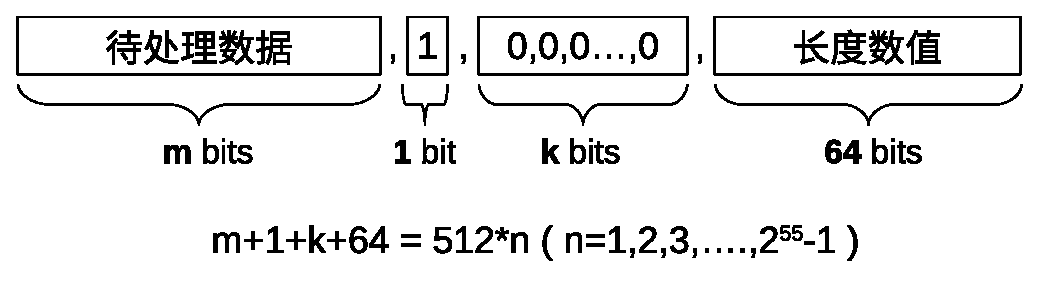
\includegraphics[width=0.7\textwidth]{./29-HMAC/figures/29-hmac-padding__CN}}
    \caption{HMAC 附加填充比特示意图}
    \label{fig:hmac-padding}
\end{figure}

下行模式下，用户无需输入数据或进行附加填充。上行模式下，若待填充数据总比特数是 512 的整数倍，则用户可配置由硬件完成 SHA 附加填充操作；若待填充数据总比特数不是 512 的整数倍，则用户只能自行完成 SHA 附加填充操作。详细步骤可参见章节 \ref{sec:hmac-process-detailed}。

\subsection{HMAC 算法结构}
HMAC 模块中应用的算法结构示意图如 \ref{fig:hmac-structure} 所示。这是 RFC 2104 中描述的标准 HMAC 算法。

\begin{figure}[ht!]
    \centering
    \fbox{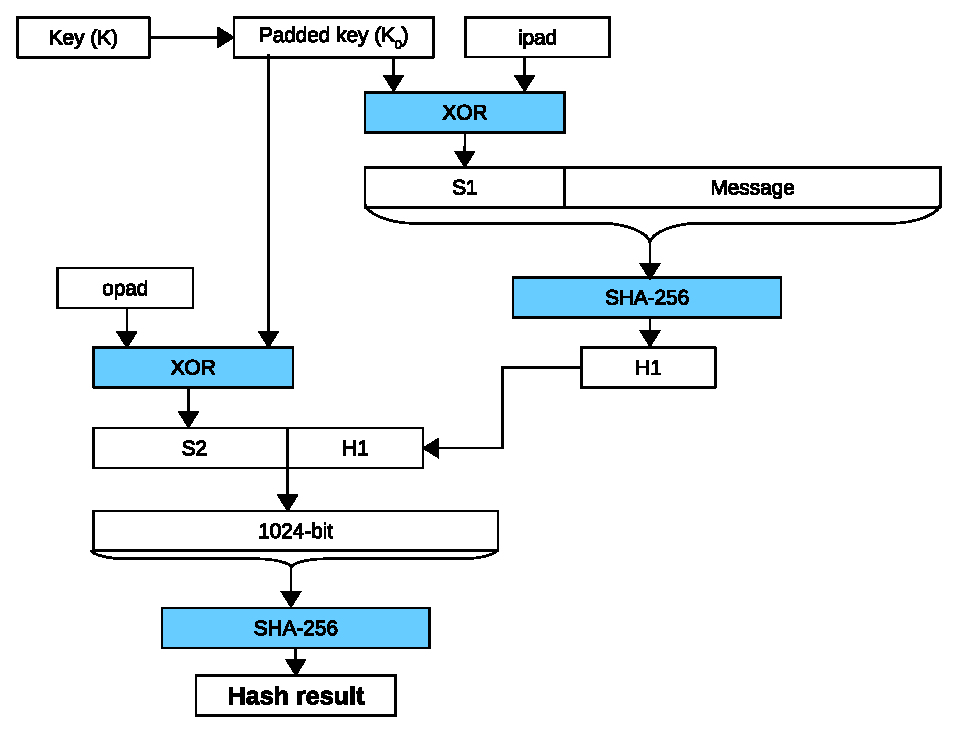
\includegraphics[width=0.8\textwidth]{./29-HMAC/figures/29-hmac-structure}}
    \caption{HMAC 结构示意图}
    \label{fig:hmac-structure}
\end{figure}

图 \ref{fig:hmac-structure} 中，
\begin{enumerate}
    \item ipad 是由 64 个 0x{}36 字节组成的 512-bit 数据块。
    \item opad 是由 64 个 0x{}5c 字节组成的 512-bit 数据块。
\end{enumerate}

\clearpage
首先，HMAC 模块在 256-bit 的密钥 K 的比特序列后附加上 256-bit 的 0 序列，得到 512-bit 的 K$_0$。再对 K$_0$ 和 ipad 进行异或运算，得到 512-bit 的 S1。将总比特数为 512 倍数的待输入数据附加到 512-bit 的 S1 数值后，使用 SHA-256 加密算法计算得到 256-bit 的 H1。

HMAC 模块通过对 K$_0$ 和 opad 进行异或运算得到 S2，将 256-bit 的 hash 计算结果附加到 512-bit 的 S2 数值后，得到 768-bit 长度的序列，使用 \ref{sec:hmac-padding} 章节中描述的 SHA 附加填充算法将该序列填充成 1024-bit 的序列，最后使用 SHA-256 加密算法计算得到的最终 hash 结果 (256-bit)。


% >>> If your module has no registers, delete sample text
%       for Sections Register Summary and Registers below <<<

%%%%%%%%%%%%%%%%%%%%%%%%
%%% Register Summary %%%
%%%%%%%%%%%%%%%%%%%%%%%%

% >>> Update the sample text below and insert
%     the info on register summary into the subfile <<<

\clearpage
\hypertarget{hmac-reg-summ}{}
\section{寄存器列表}
\label{sec:hmac-reg-summ}

本小节的所有地址均为相对于 HMAC 加速器基地址的地址偏移量（相对地址），具体基地址请见章节 \ref{mod:sysmem} \textit{\nameref{mod:sysmem}} 中的表 \ref{tab:sysmem-base-address}。

请查看章节 \hyperref[glossary-access-types]{\textit{寄存器的访问类型}}，了解“访问”列缩写的含义。

\subfile{\modulefiles/29-HMAC-reg-summ__CN}


%%%%%%%%%%%%%%%%%
%%% Registers %%%
%%%%%%%%%%%%%%%%%

% >>> Update the sample text below and insert
%      the info on registers into the subfile <<<

\clearpage
\section{寄存器}

本小节的所有地址均为相对于 HMAC 加速器基地址的地址偏移量（相对地址），具体基地址请见章节 \ref{mod:sysmem} \textit{\nameref{mod:sysmem}} 中的表 \ref{tab:sysmem-base-address}。

\subfile{\modulefiles/29-HMAC-reg__CN}


\end{document}
